\documentclass[10pt,a4paper,twoside]{book}

% Standard packages
\usepackage{palatino}
\usepackage{microtype}
\usepackage[english]{babel}
\usepackage[parfill]{parskip}
\raggedbottom
\usepackage{tocbibind}
\usepackage{xspace}
\usepackage[bottom]{footmisc}
\usepackage{tocloft}
\usepackage{fancyhdr}
\usepackage{amsmath}

% Colors
\usepackage[usenames]{color}
\definecolor{red}{rgb}{0.8,0,0}
\definecolor{blue}{rgb}{0,0,0.7}
\definecolor{lightgreen}{rgb}{0,1,0}
\definecolor{green}{rgb}{0,0.7,0}
\definecolor{gray}{rgb}{0.5,0.5,0.5}
\definecolor{yellow}{rgb}{1,1,0}

% Listings
\usepackage{listings}
\lstdefinelanguage{smalltalk}{
  string=[d]",
  comment=[s]{<}{>},
  literate=
    {^}{{$\uparrow$}}1
    {-->}{{$\longrightarrow$}}3
    {~}{{$\sim$}}1
  ,
  tabsize=5
}[keywords,comments,strings]
\lstset{
%  language=smalltalk,
%  basicstyle=\sffamily\small,
  basicstyle=\ttfamily\scriptsize,
%  commentstyle=\color{blue}\bfseries,
%  stringstyle=\color{green}\it,
  showstringspaces=false,
%  keepspaces=true,
  breaklines=true,
%  breakautoindent=true,
%  columns=fullflexible
}
\newcommand{\st}{\lstinline}
\lstnewenvironment{stcode}{
  \lstset{frame=lines}
}{}
\lstnewenvironment{stlisting}[2]{
  \lstset{
    frame=lines,
    caption={#1},
    label={listing:#2}
  }
}{}
\renewcommand{\lstlistoflistings}{
  \begingroup
    \tocfile{Listings}{lol}
  \endgroup
}


% Page geometry
\usepackage[
	papersize={6.5in,9in},
	hmargin={0.65in,0.65in},
	vmargin={0.75in,0.75in},
	ignoreheadfoot
]{geometry}

% Date formatting
\usepackage{fmtcount}
\usepackage[nodayofweek]{datetime}

% Graphics
\usepackage{graphicx}
\graphicspath{{images/}}
\DeclareGraphicsExtensions{{.pdf}}

% Constants for pdf and front page
\newcommand{\thesistitle}{Codemap}
\newcommand{\thesisauthor}{David Samuel Erni}
\newcommand{\thesissubtitle}{codemap codemap codemap codemap codemap}


% Hyperlinks
\usepackage[pdftex,colorlinks=true,pdfstartview=FitV,
 linkcolor=black,citecolor=black,urlcolor=black]{hyperref}
\hypersetup{
  a4paper,
  colorlinks,
  breaklinks=true,
  linkcolor=red,
  anchorcolor=red,
  citecolor=red,
%  pagecolor=red,
  urlcolor=magenta,
%  pagecolor=darkblue,
  pdftitle={\thesistitle},
  pdfauthor={\thesisauthor},
  pdfsubject={\thesissubtitle},
%  pdfcreator={\LaTeX},
%  pdfkeywords={\thesiskeywords},
%  bookmarksopen=true,
%  bookmarksopenlevel=2
}

%%%%%%%%%%%%%%%%%%%%%%%%%%%%%%%%%%%%%%%%%%%%%%%%%%%%%%%%%%%%%%%%%%
% Markup macros for proof-reading
\usepackage[normalem]{ulem} % for \sout
\usepackage{xcolor}
\newcommand{\ra}{$\rightarrow$}
\newcommand{\ugh}[1]{\textcolor{red}{\uwave{#1}}} % please rephrase
\newcommand{\ins}[1]{\textcolor{blue}{\uline{#1}}} % please insert
\newcommand{\del}[1]{\textcolor{red}{\sout{#1}}} % please delete
\newcommand{\chg}[2]{\textcolor{red}{\sout{#1}}{\ra}\textcolor{blue}{\uline{#2}}} % please change

%%%%%%%%%%%%%%%%%%%%%%%%%%%%%%%%%%%%%%%%%%%%%%%%%%%%%%%%%%%%%%%%%%
% Put edit comments in a really ugly standout display
\usepackage{ifthen}
\usepackage{amssymb}
\newboolean{showcomments}
\setboolean{showcomments}{true} % toggle to show or hide comments
\ifthenelse{\boolean{showcomments}}
  {\newcommand{\marking}[3]{
	% \fbox{\bfseries\sffamily\scriptsize#1}
	\fcolorbox{gray}{#3}{\bfseries\sffamily\scriptsize#1}
    {\sf\small$\blacktriangleright$\textit{#2}$\blacktriangleleft$}
    % \marginpar{\fbox{\bfseries\sffamily#1}}
   }
   %\newcommand{\version}{\emph{\scriptsize$-$Id: main.tex 25396 2009-03-12 12:37:59Z matter $-$}}
   \newcommand{\version}{}
  }
  {\newcommand{\marking}[3]{}
   \newcommand{\version}{}
  }
\newcommand{\note}[2]{\marking{#1}{#2}{yellow}}

%%%%%%%%%%%%%%%%%%%%%%%%%%%%%%%%%%%%%%%%%%%%%%%%%%%%%%%%%%%%%%%%%%
% easier referencing
\newcommand{\secref}[1]{\autoref{sec:#1}}
\newcommand{\figref}[1]{\autoref{fig:#1}}
\newcommand{\tabref}[1]{\autoref{tab:#1}}

%%%%%%%%%%%%%%%%%%%%%%%%%%%%%%%%%%%%%%%%%%%%%%%%%%%%%%%%%%%%%%%%%%
% use these to annotate your document
\newcommand{\chk}[1]{\marking{check}{#1}{lightgreen}}
\newcommand{\todo}[1]{\note{todo}{#1}}
\newcommand{\done}[1]{\note{done}{#1}}
%\newcommand{\done}[1]{}

%%%%%%%%%%%%%%%%%%%%%%%%%%%%%%%%%%%%%%%%%%%%%%%%%%%%%%%%%%%%%%%%%%
% abbreviations
\newcommand{\ie}{\emph{i.e.}\xspace}
\newcommand{\eg}{\emph{e.g.}\xspace}
\newcommand{\etc}{\emph{etc.}\xspace}
\newcommand{\cf}{\emph{cf.}\xspace}
\newcommand{\etal}{et\ al.\xspace}

%%%%%%%%%%%%%%%%%%%%%%%%%%%%%%%%%%%%%%%%%%%%%%%%%%%%%%%%%%%%%%%%%%
% names
\newcommand{\VOC}{vocabulary\xspace}
\newcommand{\VOCs}{vocabularies\xspace}
\newcommand{\cmap}{Codemap\xspace}
\newcommand{\MDS}{Multidimensional Scaling\xspace}
\newcommand{\LSI}{Latent Semantic Indexing\xspace}
\newcommand{\TOOL}{\textsc{SoftwareCartographer}\xspace}
\newcommand{\SOCA}{Software Cartography\xspace}

%%%%%%%%%%%%%%%%%%%%%%%%%%%%%%%%%%%%%%%%%%%%%%%%%%%%%%%%%%%%%%%%%%
% MAIN
%%%%%%%%%%%%%%%%%%%%%%%%%%%%%%%%%%%%%%%%%%%%%%%%%%%%%%%%%%%%%%%%%%
\begin{document}

%========================================
\frontmatter
\newcommand{\thesisemail}{deif@students.unibe.ch}
\newcommand{\thesisdate}{ 20xx}
\newcommand{\thesisurl}{\url{http://scg.unibe.ch/codemap}}

\title{\thesistitle}
\author{\thesisauthor, \thesisemail}
\date{\thesisdate}

\begin{titlepage}
  \begin{center}
    \thispagestyle{empty}
    {\bfseries\Huge\thesistitle \par}
    {\bfseries\Large\thesissubtitle \par}
    \vspace{1.1in}
    \large
    {\textbf{Masterarbeit} \\
    der Philosophisch-naturwissenschaftlichen Fakult\"{a}t \\
    der Universit\"{a}t Bern \par}
    \vspace{0.6in}
    vorgelegt von \par
     {\LARGE \thesisauthor \par}
	\todo{the date ...}     
    {\thesisdate \par}
    \vspace{1.1in}
    Leiter der Arbeit \par
    {Prof.\ Dr.\ Oscar Nierstrasz \par}
    {Adrian Kuhn \par}
    \vspace{0.6in}
    {Institut f\"ur Informatik und angewandte Mathematik \par}
  \end{center}
\end{titlepage}

\thispagestyle{empty}
\mbox{}
\vskip 10cm
\noindent Further information about this work and the tools used as well as an online version of this document can be found under the following addresses:
\vskip 11pt

\vskip 11pt
\noindent \thesisauthor\\
\thesisemail\\
\thesisurl\\
\vskip 11pt

\vskip 11pt
\noindent Software Composition Group\\
University of Bern\\
Institute of Computer Science and Applied Mathematics\\
Neubr\"uckstrasse 10\\
CH-3012 Bern\\
\url{http://scg.unibe.ch/}

%\newcommand*{\abstractname}{Abstract}
  \newenvironment{abstract}{%
        \small
        \begin{center}%
          {\bfseries \abstractname\vspace{-.5em}\vspace{0pt}}%
        \end{center}%
        \quotation
      }%
      {\endquotation}

\chapter{Abstract}
%\begin{abstract}
Software visualizations can provide a concise overview of a complex software system. Unfortunately, since software has no physical shape, there is no “natural” mapping of software to a two-dimensional space. As a consequence most visualizations tend to use a layout in which position and distance have no meaning, and consequently layout typically diverges from one visualization to another. We propose an approach to consistent layout for software visualization, called Software Cartography, in which the position of a software artifact reflects its vocabulary, and distance corresponds to similarity of vocabulary.

\todo{no we don't}
We use Latent Semantic Indexing (LSI) to map software artifacts to a vector space, and then use Multidimensional Scaling (MDS) to map this vector space down to two dimensions.


The resulting consistent layout allows us to develop a variety of thematic software maps that express very different aspects of software while making it easy to compare them. The approach is especially suitable for comparing views of evolving software, since the vocabulary of software artifacts tends to be stable over time. We present a prototype implementation of Software Cartography called \cmap, and illustrate its use with practical examples from numerous open source case studies.

\todo{user case study}
\todo{eclipse plugin, \cmap}

%\end{abstract}


\chapter{Acknowledgements}

Thank you.

\cleardoublepage
 
\tableofcontents
\label{chapter:contents}
\newpage
\cleardoublepage

%========================================
\mainmatter

%%%%%%%%%%%%%%%%%%%%%%%%%%%%%%%%%%%%%%%%%%%%%%%%%%%%%%%%%%%%%%%%%%
\chapter{Introduction}

\todo{why visualization, where it might help, what we do \dots}

Software visualization offers an attractive means to abstract from the complexity of large software systems.
A single graphic can convey a great deal of information about various aspects of a complex software system, such as its structure, the degree of coupling and cohesion, growth patterns, defect rates, and so on \cite{Dieh07a,Kien07a,Reis05a,Stor05a}.
Unfortunately, the great wealth of different visualizations that have been developed to abstract away from the complexity of software has led to yet another source of complexity: it is hard to compare different visualizations of the same software system and correlate the information they present.

We can contrast this situation with that of conventional thematic maps found in an atlas.
Different phenomena, ranging from population density to industry sectors, birth rate, or even flow of trade, are all displayed and expressed using \emph{the same consistent layout}.
It easy to correlate different kinds of information concerning the same geographical entities because they are generally presented using the same kind of layout.
This is possible because (i) there is a natural mapping of position and distance information to a two-dimensional layout\footnote{Even if we consider that the Earth is not flat on a global scale, there is still a natural mapping of position and distance to a two-dimensional layout; see the many types of cartographic projections (\eg the Mercator projection) used during centuries to do that. In fact, this is true for a large class of manifolds.}, and (ii) because by convention North is normally considered to be on the top.\footnote{The orientation of modern world maps, that is North on the top, has not always been the prevailing convention. On traditional Muslim world maps, for example, South used to be in the top. Hence, if Europe would have fallen to the Ottomans at the Battle of Vienna in 1683, all our maps might be drawn upside down by now \cite{Hite99a}.}

Software artifacts, on the other hand, have no natural layout since they have no physical location.
Distance and orientation also have no obvious meaning for software.
It is presumably for this reason that there are so many different and incomparable ways of visualizing software.
A cursory survey of recent \textsc{Softvis} and \textsc{Vissoft} publications shows that the majority of the presented visualizations feature arbitrary layout, the most common being based on alphabetical order and \emph{arbitrary hash-key order}.
(Hash-key order is what we get in most programming languages when iterating over the elements of a Set or Dictionary collection.)

Consistent layout for software would make it easier to compare visualizations of different kinds of information. But what should be the basis for positioning representations of software artifacts within a ``cartographic'' software map?
What we need is a semantically meaningful notion of position and distance for software artifacts, a spatial representation of software in a multi-dimensional space, which can then be mapped to consistent layout on the 2-dimensional visualization plane.

We propose to use \emph{vocabulary} as the most natural analogue of physical position for software artifacts, and to map these positions to a two-dimensional space as a way to achieve consistent layout for software maps.
Distance between software artifacts then corresponds to distance in their vocabulary.
Drawing from previous work \cite{Kuhn07a,Duca06c} we apply \LSI (LSI) \cite{Deer90a} to the vocabulary of a system to obtain $n$-dimensional locations, and we use \MDS (MDS) \cite{Borg05a} to obtain a consistent layout.
Finally we use cartography techniques (such as digital elevation, hill-shading and contour lines) to generate a landscape representing the frequency of topics. We call our approach \emph{\SOCA}, and call a series of visualizations \emph{Software Maps}, when they all use the same consistent layout created by our approach. 


Why should we adopt vocabulary as distance metric, and not some structural property?
First of all, vocabulary can effectively \emph{abstract} away from the technical details of source code \cite{Kuhn07a} by capturing the key domain concepts of source code. Software entities with similar vocabulary are conceptually and topically close. Lexical similarity has proven useful to detect high-level clones \cite{Marc01a} and cross-cutting concerns \cite{Pali08a} in software. Furthermore, it is known that over time vocabulary tends to be more stable than the structure of software \cite{Anto07a}, and tends to grow rather than to change \cite{Vasa07b}. Although refactorings may cause functionality to be renamed or moved, the overall vocabulary tends not to change, except as a side-effect of growth. This suggests that vocabulary will be relatively \emph{stable} in the face of change, except where significant growth occurs. As a consequence, vocabulary not only offers an intuitive notion of position that can be used to provide a consistent layout for different kinds of thematic maps, but it also provides a robust and consistent layout for mapping an evolving system. System growth can be clearly positioned with respect to old and more stable parts of the same system.

This paper is an extension of previous work, in which we first proposed \emph{\SOCA} for consistent layout of software visualizations \cite{Kuhn08b}. The main contributions of the current paper are:

\begin{itemize}
\item \emph{Improved algorithm.} In our previous work we presented a technique to create software maps given either a single release, or all releases of a system at once. In this paper we propose an improved algorithm for incremental software maps that update as new changes appear.
\item \emph{Visual stability.} In our previous work we introduced \SOCA as an approach to achieve consistent layouts for software visualization. In this paper we evaluate four open source case studies to investigate the visual stability of our approach over the evolution of a system. 
\item \emph{Desiderata for spatial representation.} We present a generalization of DeLine's desiderata for spatial software navigation~\cite{Deli05b} to spatial representation in general, and complete them with the desiderata that visual distance should have a meaningful interpretation.
\end{itemize}

%========================================
\section{Approach in a Nutshell}

%========================================
\section{Structure of the Thesis}
\todo{section x discusses blabla, section y \dots}


%%%%%%%%%%%%%%%%%%%%%%%%%%%%%%%%%%%%%%%%%%%%%%%%%%%%%%%%%%%%%%%%%%
\chapter{Related work aka what's the current situation}

% =============================================================================
\section{Previous Work}
maybe describe the software cartography prototype?

% =============================================================================
\section{Related Work}


Using \MDS to visualize information based on the metaphor of cartographic maps is by no means a novel idea. \emph{Topic maps}, as they are called, have a longstanding tradition in information visualization \cite{Ware04a}. The work in this paper was originally inspired by Michael Hermann's and Heiri Leuthold's work on the political landscapes of Switzerland \cite{Herm03a}. 

In the same way, stable layouts have a long history in information visualization, as a starting point see \eg the recent work by Frishman and Tal on online dynamic graph drawing \cite{Fris08a}. They present an online graph drawing approach, which is similar to the online pipeline presented in this work. Please refer to \autoref{sec:other} for a comparison of graph drawing and \MDS. 

ThemeScape is the best-known example of a text visualization tool that uses the metaphor of cartographic maps. 
Topics extracted from documents are organized into a visualization where visual distance correlates to topical distance and surface height corresponds to topical frequency \cite{Wise95b}. The visualization is part of a larger toolset that uses a variety of algorithms to cluster terms in documents. For laying out small document sets MDS is used; for larger document sets a proprietary algorithm, called ``Anchored Least Stress'', is used. The digital elevation model is constructed by successively layering the contributions of the contributing topical terms, similar to our approach.

In the software visualization literature however, topic maps are rarely used.
Except for the use of graph splatting in RE Toolkit by Telea \etal \cite{Tele03a}, we are unaware of their prior application in software visualization. And even in the case of the RE toolkit, the maps are not used to produce consistent layouts for thematic maps, or to visualize the evolution of a software system. 

\begin{figure}
\begin{center}
  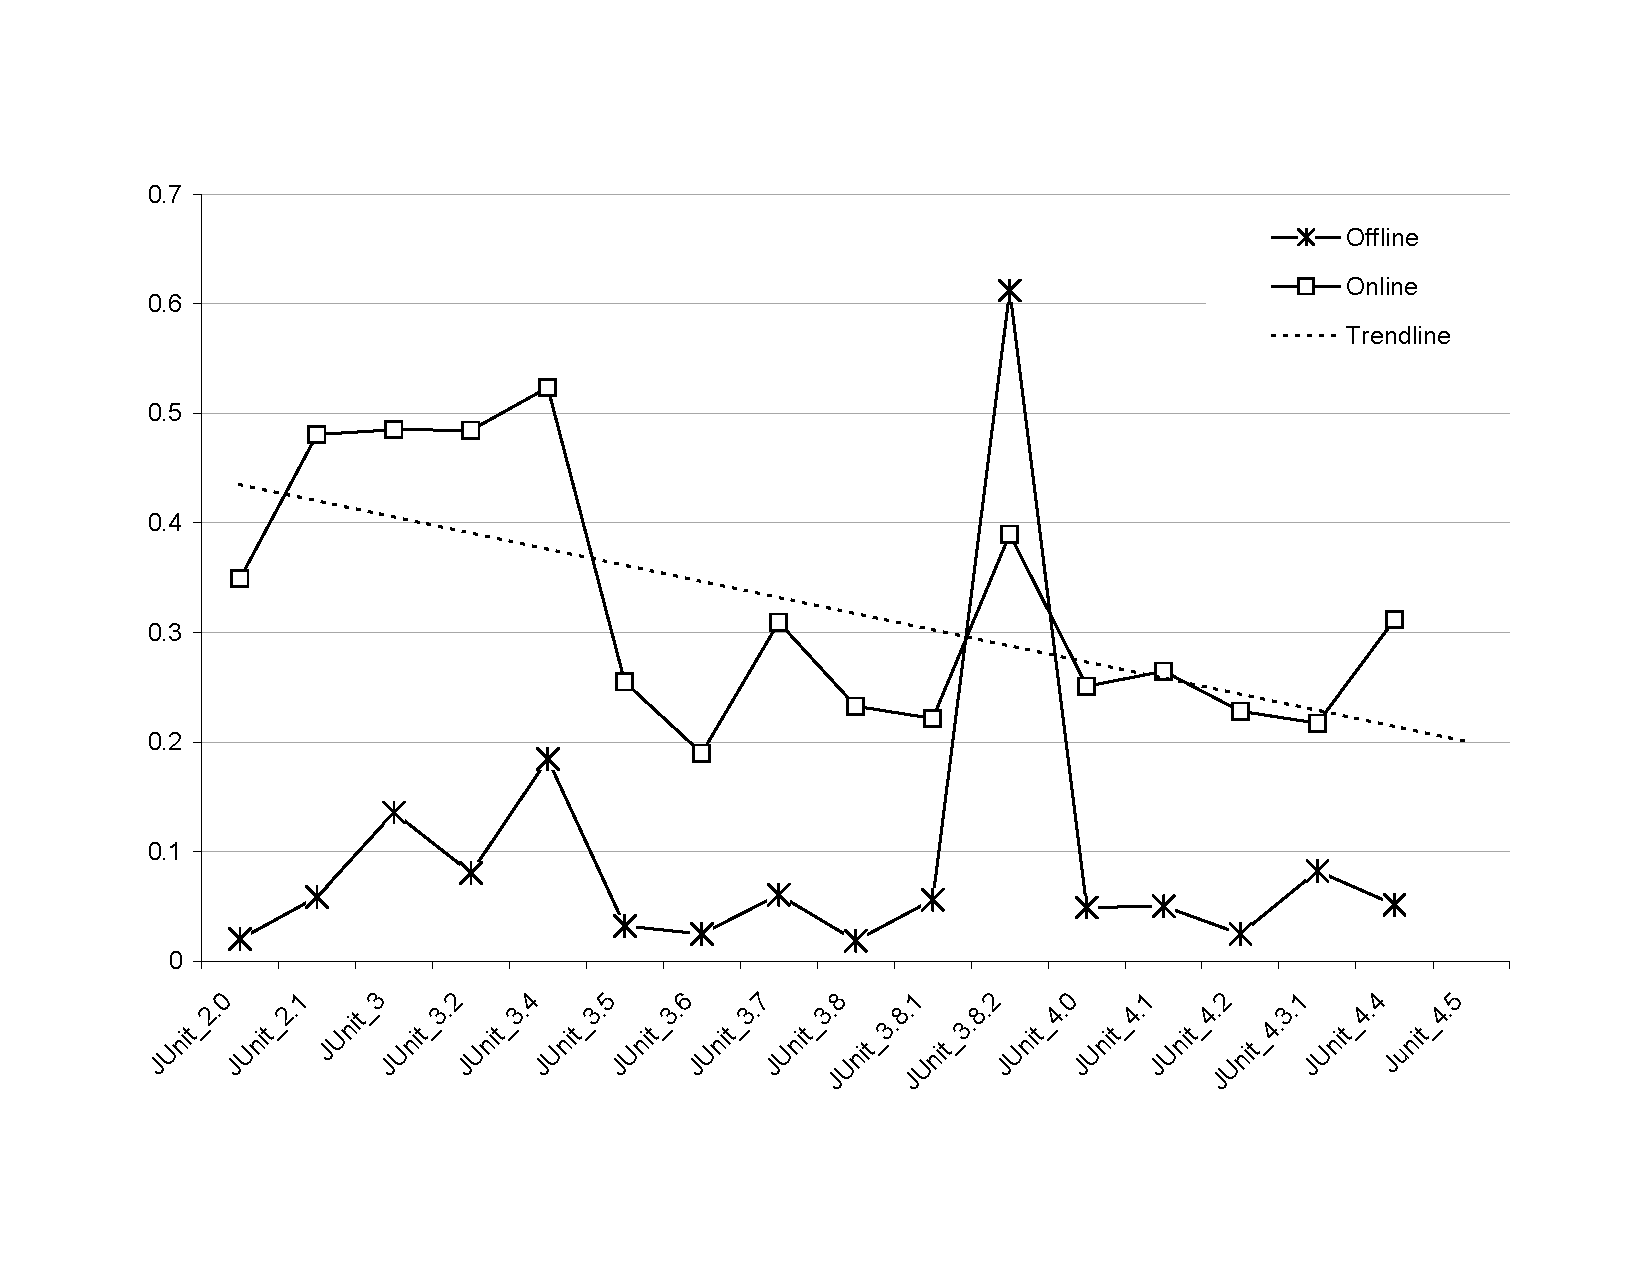
\includegraphics[width=0.7\linewidth]{junitchart.pdf}
\end{center}
    \caption{Stability chart of JUnit: the peak between release 3.8.2 and release 4.0 originates from the removal of the SwingUI classes and the addition of annotation processing classes. The online stability trends towards the offline stability.}
    \label{fig:junitchart}
\end{figure}

\begin{figure}
\begin{center}
  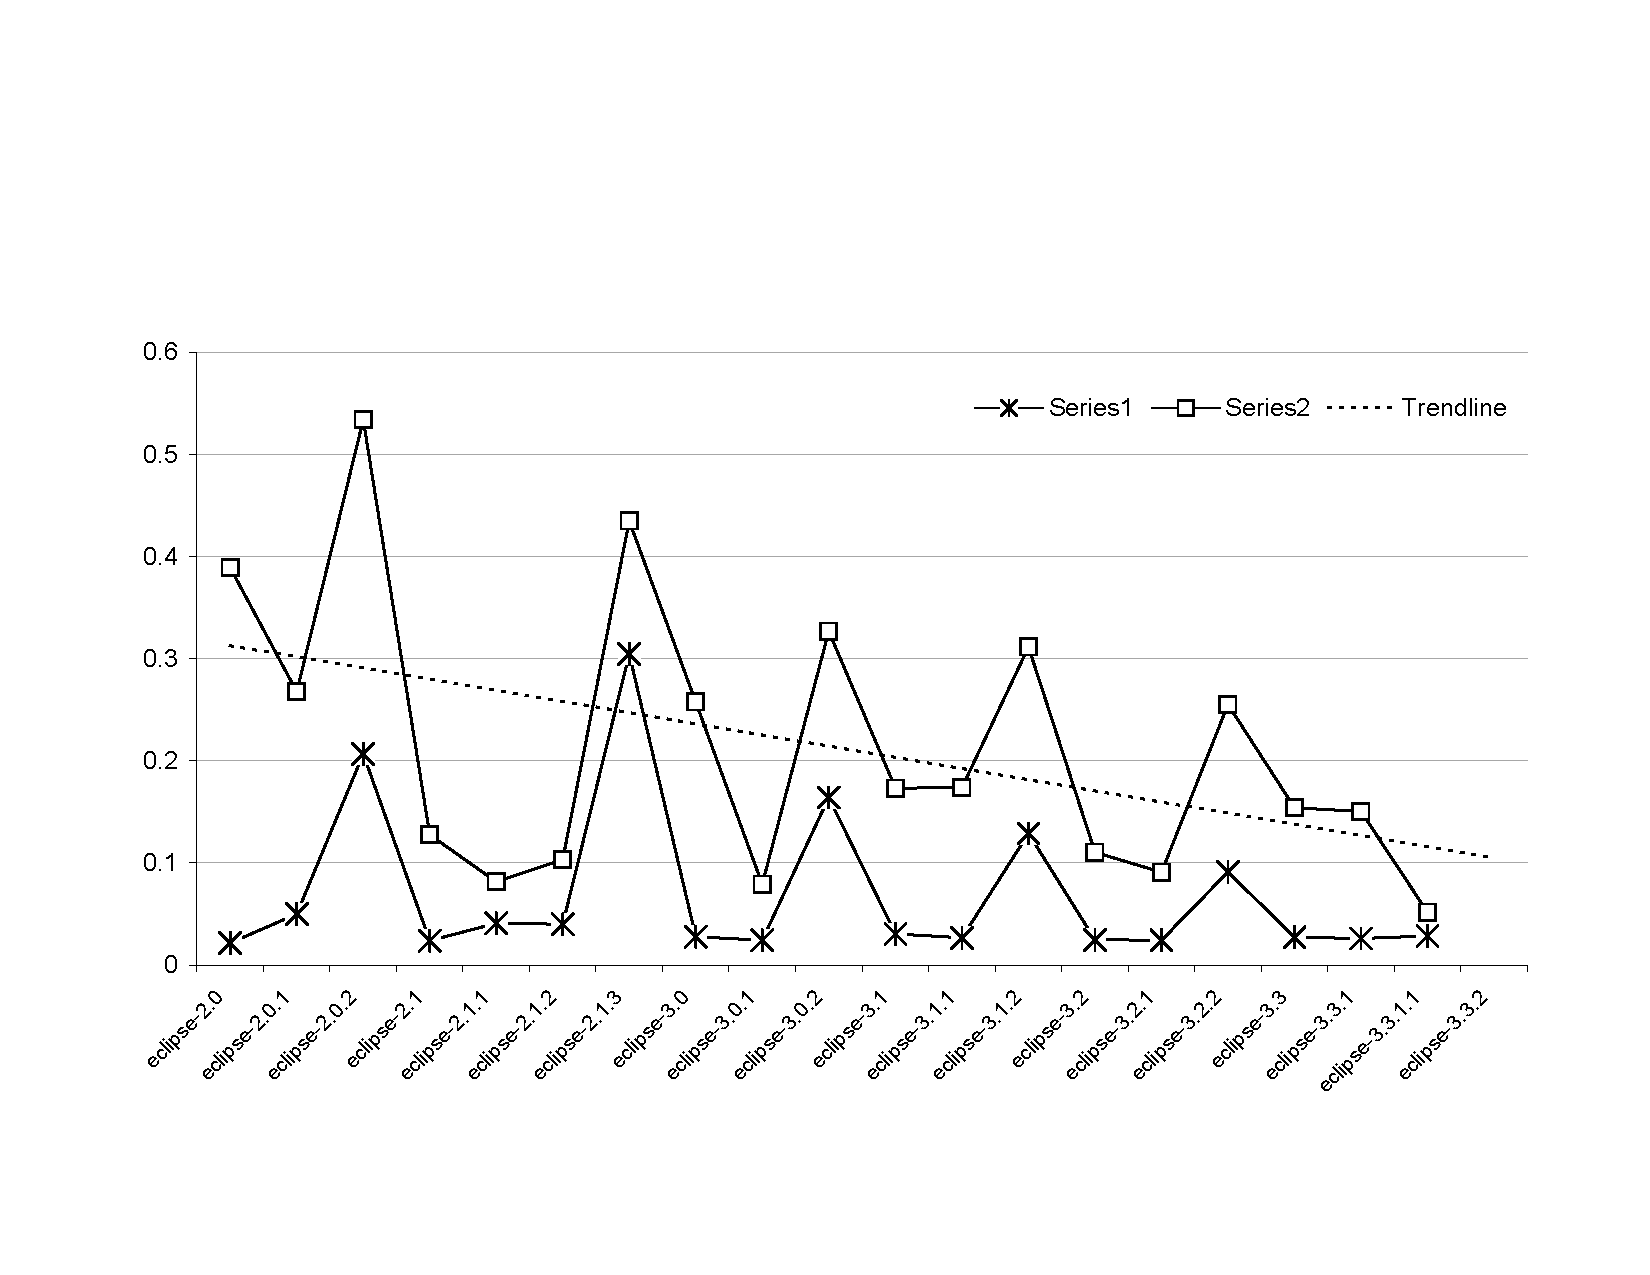
\includegraphics[width=0.85\linewidth]{eclipsechart.pdf}
\end{center}
    \caption{Stability chart of Eclipse: There are five peaks of instability, each of them correlates with a major release (\ie release 2.1. release 3.0, release 3.1, release 3.2, and release 3.3). The online stability trends towards the offline stability.}
    \label{fig:eclipsechart}
\end{figure}


\subsection{Desiderata for Spatial Representation of Software}

Robert DeLine's work on software navigation \cite{Deli05b,Deli06a} closely relates to \SOCA. His work is based on the observation that developers are consistently lost in code \cite{Deli05a} and that using textual landmarks only places a large burden on cognitive memory. He concludes the need for new visualization techniques that allow developers to use their spatial memory while navigating source code.

DeLine proposes four desiderata \cite{Deli05b} that should be satisfied by spatial software navigation: 1)~the display should show the entire program and be continuous, 2)~the display should contain visual landmarks such that developers can find parts of the program perceptually rather than relying on names, 3)~the display should remain visually stable during navigation [and evolution], and 4)~the display should be capable of showing global program information overlays other than navigation.

An ad-hoc algorithm that satisfies the first and fourth properties is presented in the same work. As distance metric between software entities (here, methods) an arbitrary chosen score is used.

Our work satisfies all above desiderata, and completes them with a fifth desideratum that visual distance should have a meaningful interpretation. The scope of \SOCA is broader than just navigation, it is also intended for reverse engineering and code comprehension in general. We can thus generalize the five desiderata for spatial representation of software as follows:

\begin{enumerate}
\item The visualization should show the entire program and be continuous.
\item The visualization should contain visualization landmarks that allow the developers to find parts of the system perceptually, rather than relying on name or other cognitive causes. 
\item The visualization should remain visually stable as the system evolves. 
\item The visualization should should be capable of showing global information overlays.
\item On the visualization, distance should have a meaningful interpretation. 
\end{enumerate}


% ~~~~~~~~~~~~~~~~~~~~~~~~~~~~~~~~~~~~~~~~~~~~~~~~~~~~~~~~~~~~~~~~~~~~~~~~~~~~~
\subsection{Other Layout Approaches used in Software Visualization}

Most software visualization layouts are based on one or multiple of the following approaches: UML diagrams, force-based graph drawing, tree-map layouts, and polymetric views.

% -------------------------------------
\emph{UML diagrams} generally employ no particular layout and do not continuously use the visualization pane. The UML standard itself does not cover the layout of diagrams. Typically a UML tool will apply an unstable graph drawing layout (\eg based on visual optimization such a reducing the number of edge crossings) when asked to automatically layout a diagram. However, this does not imply that the layout of UML diagrams is meaningless. UML diagrams are carefully created by architects, at least those made during the design process, so their layout do have a lot of meaning. If you change such a diagram and re-show it to its owner, the owner will almost suddenly complain, since he invested time in drawing the diagram a certain way! Alas, this layout process requires manual effort.

Gudenberg \etal have proposed an evolutionary approach to layout UML diagrams in which a fitness function is used to optimize various metrics (such as number of edge crossings) \cite{Gude06a}. Although the resulting layout does not reflect a distance metric, in principle the technique could be adapted to do so. Andriyevksa \etal have conducted user studies to assess the effect that different UML layout schemes have on software comprehension \cite{Andr05a}.
They report that the layout scheme that groups architecturally related classes together yields best results. They conclude that it is more important that a layout scheme convey % NB: "convey", not "conveys" (subjunctive)
a meaningful grouping of entities, rather than being aesthetically appealing. Byelas and Telea highlight related elements in a UML
% Google says 51,700 x an UML and 315,000 a UML %
diagram using a custom ``area of interest'' algorithm that connects all related elements with a blob of the same color, taking special care to minimize the number of crossings \cite{Byel06a}.
The impact of layout on their approach is not discussed.

% -------------------------------------
\emph{Graph drawing} refers to a number of techniques to layout two- and three-dimensional graphs for the purpose of information visualization \cite{Ware04a,Kauf01b}. Noack \etal offer a good starting point for applying graph drawing to software visualization \cite{Noac05a}. Jucknath-John \etal present a technique to achieve stable graph layouts over the evolution of the displayed software system \cite{Juck06a}, thus achieving consistent layout, while sidestepping the issue of reflecting meaningful position or distance metrics.

Unlike MDS, graph drawing does not map an $n$-dimensional space to two dimensions, rather it is concerned with the placement of vertices and edges such that visual properties of the output are optimized. For example, algorithms minimize the number of edge crossings or try to avoid that nodes overlap each other. Even though, the standard force-based layouts can consider edge weights (which can be seen as a distance metric), edges with the same weight may have different length on the visualization pane depending on the connectedness of the graph at that position. Furthermore, the resulting placement is not continuos. The void between vertices is not continuous spectrum of metric locations, as is the case with an MDS layout.

\emph{Graph splatting} is a variation of graph drawing, which produced visualizations that are very similar to thematic maps \cite{Lier03a}. Graph splatting represents the layout of graph drawing algorithms as a continuous scalar field. Graph splatting combines the layout of graph drawing with the rendering of thematic maps. Each vertex contributes to the field with a Gaussian shaped basis function. The elevation of the field thus represents the density of the graph layout at that position. Telea \etal apply Graph splatting in their RE toolkit to visualize software systems \cite{Tele03a}. However, they are not concerned with stable layouts. Each run of their tool may yield a different layout.

% -------------------------------------
\emph{Treemaps} represent tree-structured information using nested rectangles \cite{Ware04a}.
Though treemaps make continuous use of the visualization pane, the interpretation of position and distance is implementation dependent. Classical treemap implementations are known to produce very narrow and thus distorted rectangles. Balzer \etal proposed a modification of the classical treemap layout using Voronoi tessellation \cite{Balz05a}. Their approach creates aesthetically more appealing treemaps, reducing the number of narrow tessels. There are some treemap variations (\eg the strip layout or the squarified layout) that can, and do, order the nodes depending on a metric. However, nodes are typically ordered on a local level only, not taking into account the global co-location of bordering leaf nodes contained in nodes that touch at a higher level. Many treemaps found in software visualization literature are even applied with arbitrary order of nodes, such as alphanumeric order of class names. 

\emph{Polymetric views} visualize software systems by mapping different software metrics on the visual properties of box-and-arrow diagrams \cite{Lanz03d,Lanz06a}. Many polymetric views are ordered by the 
value of a given software metric, so that relevant items appear first (whatever first means, given the 
layout). Such an order is more meaningful then alphabetic (or worse, hash-key ordering), but on the other hand only as stable as the used metric. The System Complexity view is by far the most popular polymetric view, and is often used as a base layout where our requirements for stability and consistence apply (see \eg \cite{Gree06a}). The layout of System Complexity uses graph drawing on inheritance relations, and orders the top-level classes as well as each layer of subclasses by class names. Such a layout does not meet our desiderate for a stable and consistent layout.
   
% ~~~~~~~~~~~~~~~~~~~~~~~~~~~~~~~~~~~~~~~~~~~~~~~~~~~~~~~~~~~~~~~~~~~~~~~~~~~~~
\subsection{ More Cartography Metaphors in Software Visualization}\label{sec:other}

A number of tools have adopted metaphors from cartography in recent years to visualize software.
Usually these approaches are integrated in a tool with in an interactive, explorative interface and often feature three-dimensional visualizations. None of these approaches satisfies DeLine's desiderata.

MetricView is an exploratory environment featuring UML diagram visualizations \cite{Term05a}. The third dimension is used to extend UML with polymetric views \cite{Lanz03d}.
The diagrams use arbitrary layout, so do not reflect meaningful distance or position.

White Coats is an explorative environment also based on the notion of polymetric views \cite{Mesn05b}. The visualizations are three-dimensional with position and visual-distance of entities given by selected metrics. However they do not incorporate the notion of a consistent layout.

CGA Call Graph Analyser is an explorative environment that visualizes a combination of function call graph and nested modules structure \cite{Bohn07a}. The tool employs a 2$\frac{1}{2}$-dimensional approach. To our best knowledge, their visualizations use an arbitrary layout.

CodeCity is an explorative environment building on the city metaphor \cite{Wett07b}. CodeCity employs the nesting level of packages for their city's elevation model, and uses a modified tree layout to position the entities, \ie packages and classes. Within a package, elements are ordered by size of the element's visual representation. Hence, when changing the metrics mapped on width and height, the overall layout of the city changes, and thus, the consistent layout breaks.

VERSO is an explorative environment that is also based on the city metaphor \cite{Lang05a}. Similar to CodeCity, VERSO employs a treemap layout to position their elements. Within a package, elements are either ordered by their color or by first appearance in the system's history. As the leaf elements have all the same base size, changing this setting does not change the overall layout. Hence, they provide consistent layout, however within the spatial limitations of the classical treemap layout. 

%%%%%%%%%%%%%%%%%%%%%%%%%%%%%%%%%%%%%%%%%%%%%%%%%%%%%%%%%%%%%%%%%%
\chapter{\SOCA}

\todo{what is software cartography, how do we do it }

% =============================================================================
\section{On the Choice of Vocabulary}

The decision to use a distance based on lexical similarity does, indeed, create a distribution of distances that should not change a lot in time. This is because programmers will not use a completely new set of lexical tokens in each new version of the software. In fact, it has been shown that over time vocabulary tends to be more stable than the structure of software \cite{Anto07a}. However, this also will create software maps that naturally only can show how items are similar from a lexical point of view.

The map layout as presented in this work can, of course, be used to see how items are related from the point of view of some other distance, such as considering structural similarity, similarity with regard to a complexity or testability metric. In that case, the distance may vary a lot over time during the evolution of a product, and this will create unstable layouts. The focus of this work, however, is the creation of maps that help programmers to establish a stable mental model of their software system under work. In any case, if maps  based on other metrics are ever to be used in conjunction with vocabulary-based \SOCA maps, we strongly recommend to visually distinguish them by using another rendering scheme. This helps to reduce the likeliness that programmers confuse the spatial layout of these other maps, with the mental model acquired through the use of \SOCA maps. 

As mentioned in the introduction, \SOCA is vocabulary-based because vocabulary can effectively \emph{abstract} away from the technical details of source code \cite{Kuhn07a} by capturing the key domain concepts of source code. The assumption being that software entities with similar vocabulary are conceptually and topically close. Consider, for example, programming languages and software where name overloading is applied. Even though overloaded methods differ in their implementation strategy, they will typically implement the same concept using the same vocabulary. In fact, lexical similarity has proven useful to detect high-level clones \cite{Marc01a} and cross-cutting concerns \cite{Pali08a} in software.  

Due to name scoping, semantically different scopes can have identical names with different meanings. Consider, for example, two large functions having mostly identifiers such as i, j, prev, next, end, stop, flag, \dots;  the one does some matrix computations, while the other is a hash-table implementation. Without the application of \LSI (\secref{lsi}) the two would be classified as being very similar, while this is clearly not true from a developer's perspective. \LSI, however, can identify words that have different meaning depending on their context. LSI has the ability to resolve certain synonymy and polysemy \cite{Deer90a}.


Although refactorings may cause functionality to be renamed or moved, the overall vocabulary tends not to change, except as a side-effect of growth \cite{Zhan08a,Vasa07b}. Consider the example of a rename refactoring. Two effects may occur. 
In the first case, all occurrences of a symbol are replaced with new symbol. This will not affect the map, since both lexical similarity and LSI are based on statistical analysis only. Replacing all occurrences of one term with a new term is, from the point of these IR technologies, a null operation. In the second case, some occurrences of a symbol are replaced with another symbol which is already used. This will indeed affect the layout of the map. Given that the new name was well chosen by the programmer, the new layout constitutes a better representation of the system. On the other hand, if the new name is a bad choice, the new layout is flawed. However, what constitutes bad naming is not merely a matter of taste. Approaches that combine vocabulary with structural information can indeed assess the quality of naming. Please refer to H\o{}st's recent work on debugging method names for further reading \cite{Hoes09a}.

Not considered in the present work is the relative weight of different lexical tokens. For example, it seems reasonable to weight local identifiers differently than identifiers in top-level namespaces. Also, one may treat names coming from library functions different from the ones coming from the actual user code. Given the absence of evaluation benchmarks, we decided to use equal weighting for all lexical token. Also, preliminary experiments with different weighting schemes indicate that relative weights below boost level, \ie below a factor of 10, do often not significantly affect the overall layout.

In this section we present the techniques that are used to achieve a consistent layout for software maps. We present two variations of \SOCA, an \emph{offline} algorithm that requires that all releases of a software system are available upfront, and an improved \emph{online} algorithm that updates the layout incrementally as new releases of the system appear. 

The general approach of \SOCA, as illustrated in \autoref{fig:soca}, is as follows:
\begin{enumerate}
\item We parse the vocabulary of source files into term-frequency histograms. All text found in raw source code is taken into account, including not only identifiers but also comments and literals.
\item We transform the term-frequency histograms using \LSI (LSI) \cite{Deer90a}, an information retrieval technique that resolves synonymy and polysemy. 
\item We use \MDS (MDS) \cite{Borg05a} to map the term-frequency histograms onto the 2D visualization pane. This preserves the lexical co-relation of source files as well as possible.
\item We use cartographic visualization techniques to render an aesthetically appealing landscape.
\end{enumerate}

Possible applications of \SOCA in the software development process are, \dots

\begin{itemize}
\item \dots to navigate within a software system, be it for development or analysis.
\item \dots to relate different metrics to each other, \eg search results and bug prediction.
\item \dots to stay in touch with other developers of your team, by showing open files of other developers.
\item \dots to understand a system’s domain upon first contact.
\item \dots to explore a system during reverse engineering.
\end{itemize}

\noindent We implemented a prototype of our approach, \TOOL, which is available as an open source project. \TOOL was originally programmed in Smalltalk, in the mean time development has been moved to Java. \TOOL is available as an Eclipse plug-in\footnote{\url{http://scg.unibe.ch/codemap}}.

% =============================================================================
\section{Implementation}

% ~~~~~~~~~~~~~~~~~~~~~~~~~~~~~~~~~~~~~~~~~~~~~~~~~~~~~~~~~~~~~~~~~~~~~~~~~~~~~
\subsection{Lexical Similarity between Source Files}

As motivated in the introduction, the distance between software entities on the map is based on the lexical similarity of source files. Lexical similarity is an Information Retrieval (IR) technique based on the vocabulary of text files. Formally, lexical similarity is defined as the cosine between the term frequency vectors of two text documents. That is, the more terms (\ie identifiers names and operators, but also words in comments) two source files share, the closer they are on the map. 

First, the raw source files are split into terms. Then a matrix is created, which lists for each document the occurrences of terms. Typically, the vocabulary of source code consists of 500--20'000 terms. In fact, studies have shown that the relation between term count and software size follows a power law \cite{Zhan08a}. For this work, we consider all text found in raw source files as terms. This includes class names, methods names, parameter names, local variables names, names of invoked methods, but also words found in comments and literal values. Identifiers are further preprocessed by splitting up the camel-case name convention which is predominantly used in Java source code. Note that since our approach is based on raw text, any programming language that uses textual source files might  be processed.

In a next step, \LSI \cite{Deer90a} is applied to reduce the rank of the term-document matrix to about 50 dimensions. LSI is able to resolve issues of synonymy and polysemy without the use of predefined dictionaries. This is advantageous for the vocabulary of source code which often deviates from common English usage. For more details on \LSI and lexical similarity, please refer to our previous work on software clustering \cite{Kuhn07a}.

% ~~~~~~~~~~~~~~~~~~~~~~~~~~~~~~~~~~~~~~~~~~~~~~~~~~~~~~~~~~~~~~~~~~~~~~~~~~~~~~
\subsection{Hill-shading and Contour Lines}
In \figref{steps} we see an overview of the steps taken to render a software map.
To make our map more aesthetically appealing, we add a touch of three-dimensionality.

The hill-shading algorithm is well-known in geographic visualization. It adds hill shades to a map \cite{Sloc05a}. The algorithm works on a distinct height model (digital elevation model) rather than on trigonometric data vetor date: each pixel has an assigned z-value, its height. 

The digital elevation model of \TOOL is is a simple matrix with discrete height information for all pixels of the visualization plane. As illustrated on Figure~\ref{fig:dem}, each element (ie source file of class) is represented by the a hill who's height corresponds to the element's KLOC size. The shape of the hill is determined using a normal distribution function. To avoid that closely located element hide each other, the elevation of all individual elements is summed up.


The hill-shading algorithm renders a three-dimensional looking surface by determining an illumination value for each cell in that matrix. It does this by assuming a hypothetical light source and calculating the illumination value for each cell in relation to its neighboring cells.

Eventually, we add contour lines. Drawing contour lines on maps is a very common technique in cartography. Contour lines make elevation more evident then hill-shading alone. Since almost all real world maps make use contour lines, maps with contour lines are very familiar to the user.


% ~~~~~~~~~~~~~~~~~~~~~~~~~~~~~~~~~~~~~~~~~~~~~~~~~~~~~~~~~~~~~~~~~~~~~~~~~~~~~~
\subsection{Labeling}

A map without labels is of little use. On a software map, all entities are labeled with their name (class or file name).

Labeling is a non-trivial problem, we must make sure that no two labels overlap. Also labels should not overlap important landmarks. Most labeling approaching are semi-automatic and need manual adjustment, an optimal labeling algorithm does not exist \cite{Sloc05a}. For locations that are near to each other it is difficult to place the labels so that they do not overlap and hide each other. For software maps it is even harder due to often long class names and clusters of closely related classes.

The examples given in this paper show only the most important class names. \TOOL uses fully-automatic, greedy brute-force approach. Labels are placed either to the top left, top right, bottom left, or bottom right of their element. Smallers labels are omitted if covered by a larger label. Eventually, among all layouts, the one where most labels are shown is chosen.


% =============================================================================
\section{On different Layout Algorithms}
\todo{describe the evolution of layout algorithms}


% =============================================================================
\section{Examples}
\todo{provide some nice examples}

In this section we present examples of \SOCA. The first example visualizes the evolution of a small software system. The second example shows an overview of six open-source systems. As the third example, we provide two thematic overlays of the same software map.

% ~~~~~~~~~~~~~~~~~~~~~~~~~~~~~~~~~~~~~~~~~~~~~~~~~~~~~~~~~~~~~~~~~~~~~~~~~~~~~~
\subsection{The Evolution of Ludo}

Figure~\ref{fig:ludo} shows the complete history of the Ludo system, consisting of four iterations. Ludo is used in a first year programming course to teach iterative development (please mail the first author to get the sources). The 4th iteration is the largest with 30 classes and a total size of 3-4 KLOC. We selected Ludo because in each iteration, a crucial part of the final system is added. 

\begin{itemize}

\item The first map (\autoref{fig:ludo}, leftmost) shows the initial prototype. This iteration implements the board as a linked list of squares. Most classes are located in the south-western quadrant. The remaining space is occupied by ocean, nothing else has been implemented so far.

\item In the second iteration (\autoref{fig:ludo}, second to the left) the board class is extended with a factory class. In order to support players and stones, a few new classes and tests for future game rules are added. On the new map the test classes are positioned in the north-eastern quadrant, opposite to the other classes. This indicates that the newly added test classes implement a novel feature (\ie testing of the game's ``business rules'') and are thus not related to the factory's domain of board initialization. 

\item During the third iteration (\autoref{fig:ludo}, second to the right) the actual game rules are implemented. Most rules are implemented in the {\tt Square} and {\tt Ludo} class, thus their mountain rises. In the south-west, we can notice that, although the {\tt BoardFactory} has been renamed to {\tt LudoFactory}, its position on the map has not changed considerably. 

\item The fourth map (\autoref{fig:ludo}, rightmost) shows the last iteration. A user interface and a printer class have been added. Since both of them depend on most previous parts of the application they are located in the middle of the map. Since the new UI classes use vocabulary from all parts of the system, the islands are joined into a continent.

\end{itemize}

The layout of elements remains stable over all four iterations.  For example, Board/LudoFactory is on all four views located in the south-western quadrant. This is due to LSI's robustness in the face of synonymy and polysemy; as a consequence most renamings do not significantly change the vocabulary of a software artifact \cite{Kuhn07a}.

\newlength{\figwidth}
\setlength{\figwidth}{0.32\textwidth}
\begin{figure*}
\begin{center}
\begin{minipage}{\figwidth}
\begin{center}
  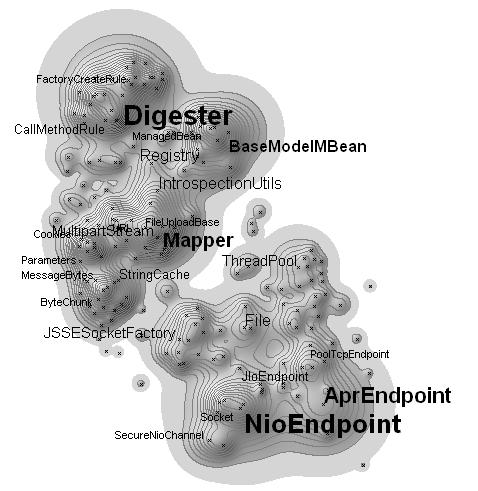
\includegraphics[width=\figwidth]{apache-tomcat-bw.png}\\
  Apache Tomcat
\end{center}
\end{minipage}~
\begin{minipage}{\figwidth}
\begin{center}
  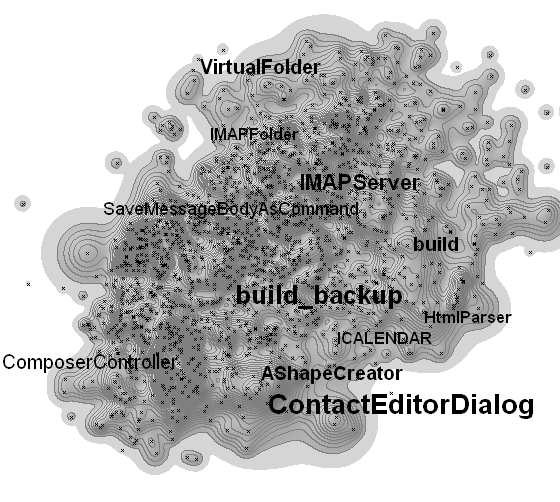
\includegraphics[width=\figwidth]{columba-bw.png}\\
  Columba
\end{center}
\end{minipage}
\begin{minipage}{\figwidth}
\begin{center}
  
\includegraphics[width=\figwidth]{google-taglib-bw.png}\\
  Google Taglib
\end{center}
\end{minipage}
\begin{minipage}{\figwidth}
\begin{center}
  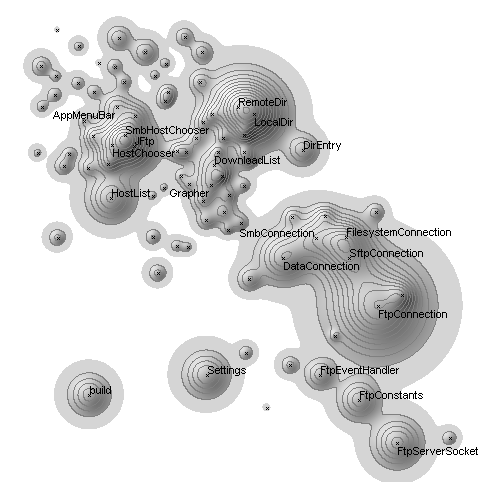
\includegraphics[width=\figwidth]{j-ftp-bw.png}\\
  JFtp
\end{center}
\end{minipage}
\begin{minipage}{\figwidth}
\begin{center}
  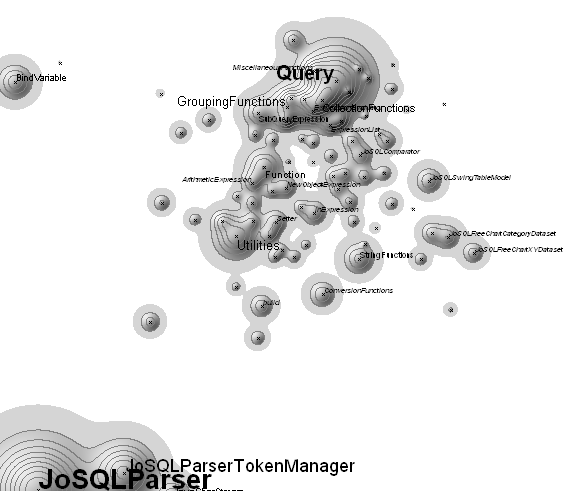
\includegraphics[width=\figwidth]{JoSQL-bw.png}\\
  JoSQL
\end{center}
\end{minipage}
\begin{minipage}{\figwidth}
\begin{center}
  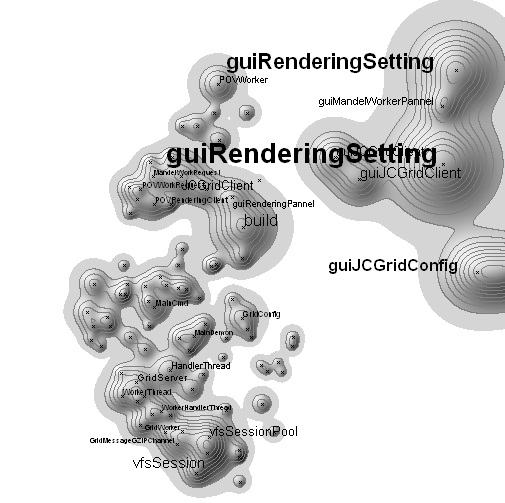
\includegraphics[width=\figwidth]{jcgrid-bw.png}\\
  JCGrid
\end{center}
\end{minipage}
\end{center}
\vspace{1ex}
    \caption{Overview of the software maps of six open source systems. Each map reveals a distinct spatial structure. When consequently applied to every visualization, the consistent layout may soon turn into the system's iconic fingerprint. An engineer might \eg point to the top left map and say: ``Look, this huge {\tt Digester} peninsula in the north, that must be Tomcat. I know it from last year's code review.''.
    }
    \label{fig:fullpage}
\end{figure*} 

% ~~~~~~~~~~~~~~~~~~~~~~~~~~~~~~~~~~~~~~~~~~~~~~~~~~~~~~~~~~~~~~~~~~~~~~~~~~~~~~
\subsection{Open-source examples}

We applied the \SOCA approach to all systems listed in the field study by Cabral and Marques \cite{Cabr07a}. They list 32 systems, including 4 of each type of application (Standalone, Server, Server Applications, Libraries) and selected programming language (Java, .NET).  

Figure \ref{fig:fullpage} shows the software map for six of these systems: Apache Tomcat, Columba, Google Taglib, JFtp, JCGrid and JoSQL. Each system reveals a distinct spatial structure. Some fall apart into many islands, like JFtp, whereas others cluster into one (or possibly two) large contents, like Columba and Apache Tomcat. The 36 case-studies raised interesting questions for future work regarding the correlation between a system's layout and code quality. For example, do large continents indicate bad modularizations? Or, do archipelagoes indicate low coupling?

%Each system's size in TLC and KLOC is listed in Table~\ref{tab:six}.

%\begin{table}[htdp]
%\begin{center}
%\begin{tabular}{l|rr}
%\textbf{System} & \textbf{\# Top-level} & \textbf{KLOC} \\
% & \textbf{classes} & \\
%\hline
%Apache Tomcat & 162 & 14'700 \\
%Columba & 1'549 & 53'500 \\
%Google Taglib & 20 & 940 \\ 
%JFtp & 78 & 3'470 \\
%JCGrid & 94 & 3'630 \\
%JoSQL & 83 & 6'480 \\
%\end{tabular}
%\end{center}
%\vspace{1ex}
%\caption{Statistics of the six systems in Figure~\ref{fig:fullpage}. \AK{Are you sure this is KLOC? Does Google Taglib really have 0.9 million(!) lines of code in 20 classes only?}
%}
%\label{tab:six}
%\end{table}

% ~~~~~~~~~~~~~~~~~~~~~~~~~~~~~~~~~~~~~~~~~~~~~~~~~~~~~~~~~~~~~~~~~~~~~~~~~~~~~~
\subsection{Thematic cartography examples}

\begin{figure}
\begin{center}
\begin{minipage}{1.4\figwidth}
\begin{center}
  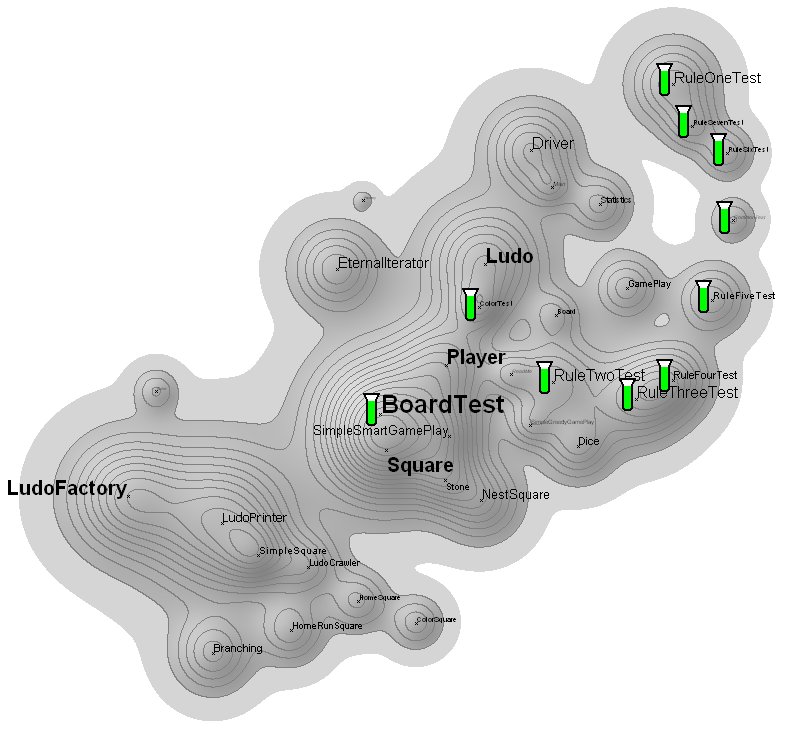
\includegraphics[width=1.4\figwidth]{ludo-v4-testtubes.png}
\end{center}
\end{minipage}
\begin{minipage}{1.4\figwidth}
\begin{center}
  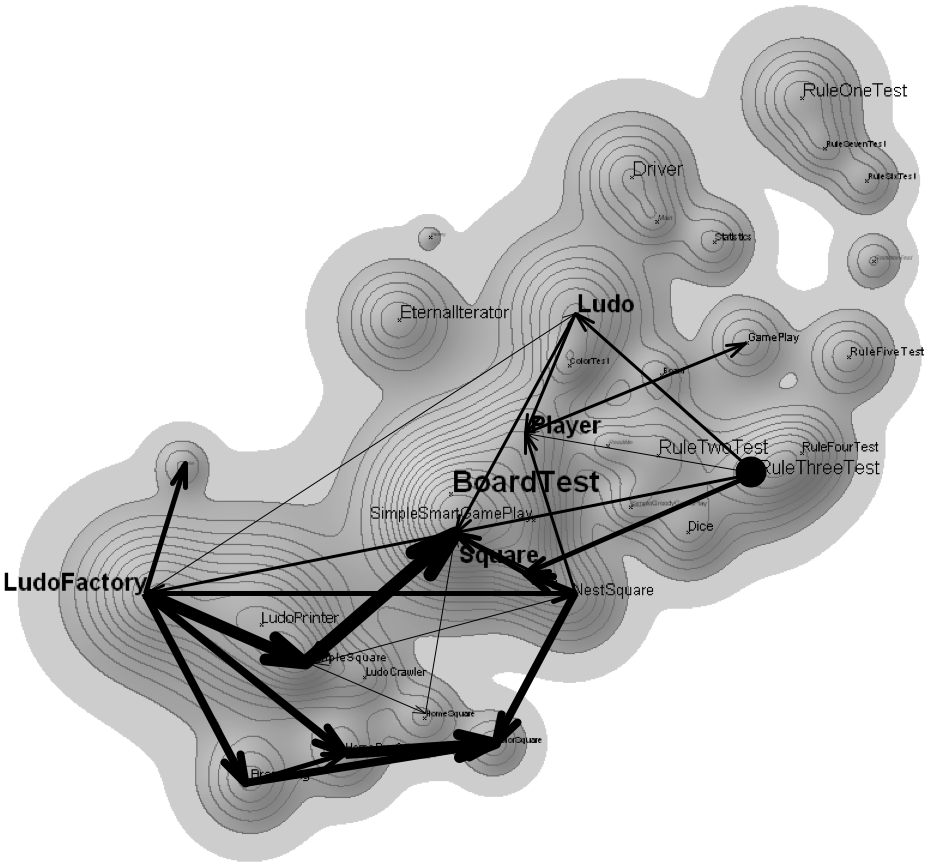
\includegraphics[width=1.4\figwidth]{ludo-v4-testexecution.png}
\end{center}
\end{minipage}
\end{center}
    \caption{Software maps with thematic overlay: (left) glyphs are drawn on top of the map, to display additional information. Each test tube glyph indicates the location of unit test case, (right) invocation edges are drawn on top of the map, showing the trace of executing the {\tt RuleThreeTest} test case.}
    \label{fig:mock}
\end{figure}

Software maps can be used as canvas for more specialized visualizations of the same system. In the following, we provide two thematic visualization of the Ludo system that might benefit from consistent layout. (The maps in this subsection are mockups, not yet fully supported by \TOOL.)

\begin{itemize}

\item Boccuzzo and Gall present a set of metaphors for the visual shape of entities \cite{Bocc07a}. They use simple and well-known graphical elements from daily life, such as houses and tables. However they use conventional albeit arbitrary layouts, where the distribution of glyphs often does not bear a meaningful interpretation. The first map in Figure~\ref{fig:mock} (on the left) employs their technique on top of a software map, using test tubes to indicate the distribution of test cases.

\item Greevy \etal present a three-dimensional variation of System Complexity View to visualize a System's dynamic runtime state \cite{Gree05d}. They connect classes with edges representing method invocation, and stack boxes on top of each other to represent a class's instances.
Since System Complexity Views do not capture any notion of position, the lengths of their invocation edges do not express any real sense of distance.

Figure~\ref{fig:mock} (on the right) employs their approach on top of a software map, drawing invocation edges in a two-dimensional plane.
Here the distances have an interpretation in terms of lexical distance, so the lengths of invocation edges are meaningful.
A short edge indicates that closely related artifacts are invoking each other, whereas long edges indicate a ``long-distance call'' to a lexically unrelated class.

\end{itemize}


%%%%%%%%%%%%%%%%%%%%%%%%%%%%%%%%%%%%%%%%%%%%%%%%%%%%%%%%%%%%%%%%%%
\chapter{Codemap}

\todo{describe the eclipse plugin}

% =============================================================================
\section{plugin structure}

% ~~~~~~~~~~~~~~~~~~~~~~~~~~~~~~~~~~~~~~~~~~~~~~~~~~~~~~~~~~~~~~~~~~~~~~~~~~~~~~
\subsection{the menubar ...}



%%%%%%%%%%%%%%%%%%%%%%%%%%%%%%%%%%%%%%%%%%%%%%%%%%%%%%%%%%%%%%%%%%
\chapter{Case Study}

%========================================
\section{Studies of different layouts}

%========================================
\section{Study on stability over time}

%========================================
\section{Usability studies}
\todo{or maybe not}
%%%%%%%%%%%%%%%%%%%%%%%%%%%%%%%%%%%%%%%%%%%%%%%%%%%%%%%%%%%%%%%%%%
\chapter{Discussion}
the blabla

%%%%%%%%%%%%%%%%%%%%%%%%%%%%%%%%%%%%%%%%%%%%%%%%%%%%%%%%%%%%%%%%%%
\chapter{Conclusion}

This paper presents \SOCA, a spatial representation of software. Our approach visualizes software entities using a consistent layout. Software maps present the entire program and are continuous. Software maps contain visual landmarks that allow developers to find parts of the system perceptually rather then relying on conceptual clues, \eg names. Since all software maps of a system use the same layout, maps with thematic overlays can be compared to each other.

The layout of software maps is based on the lexical similarity of software entities. Our algorithm uses \LSI to position software entities in an multi-dimensional space, and \MDS to map these positions on a two-dimensional display. Software maps can be generated to depict evolution of a software system over time. We evaluated the visual stability of iteratively generated maps considering four open source case studies.

In spite of the aesthetic appeal of hill shading and contour lines, the main contribution of this paper is not the cartographic look of software maps. The main contribution of \SOCA is (i) that cartographic position reflects topical distance of software entities, and (ii) that consistent layout allows different software maps to be easily compared.
In this way, software maps reflect world maps in an atlas that exploit the same consistent layout to depict various kinds of thematic information about geographical sites.

We have presented several examples to illustrate the usefulness of software maps to depict the evolution of software systems, and to serve as a background for thematic visualizations.
The examples have been produced using \TOOL, a proof-of-concept tool that implements our technique.

As future work, we can identify the following promising directions:
\begin{itemize}
  \item Software maps at present are largely static.
  We envision a more interactive environment in which the user can ``zoom and pan'' through the landscape to see features in closer detail, or navigate to other views of the software.
  \item Selectively displaying features would make the environment more attractive for navigation. Instead of generating all the labels and thematic widgets up-front, users can annotate the map, adding comments and waymarks as they perform their tasks.
  \item Orientation and layout are presently consistent for a single project only.
  We would like to investigate the usefulness of conventions for establishing consistent layout and orientation (\ie ``testing'' is North-East) that will work across multiple projects, possibly within a reasonably well-defined domain.
  \item We plan to perform an empirical user study to evaluate the application of \SOCA for software comprehension and reverse engineering, but also for source code navigation in development environments.
\end{itemize}


% ================================================================================
\section{Future Work}
it's always nice to tell someone else to clean up all the cruft.

% ================================================================================
\section{Lessons Learned}

testing

%========================================
\appendix
\chapter{Appendix stuff}

%\clearpage
%\cleardoublepage




\listoffigures
\lstlistoflistings
\listoftables
\clearpage

%========================================
\backmatter
%\renewcommand{\bibname}{Works Cited}
\bibliographystyle{plain}
\bibliography{bib/scg,bib/thesis,bib/local}


\end{document}
